Para la experimentación se utilizó una máquina Desktop Intel(R) Core(TM) i5-4570T CPU @ 2.90GHz, 5.7G Ram, con DB: 5.5.46-MariaDB-1ubuntu0.14.04.2.

El análisis que se realiza de los resultados obtenidos es comparando la calidad de los resultados de los algoritmos discutidos en \autoref{chap:desarrollo}, sobre las bases de datos de \autoref{chap:busquedas}. Con el objetivo de evaluar las propuestas algorítmicas, se consideraron los siguientes métodos:

\begin{itemize}
\item{$alg1$} PAC(C-HAC / selección simple)
\item{$alg2$} PAC(BOBO-10 / selección simple)
\item{$alg3$} PAC(BOBO-10 / selección proporcional)
\item{$alg4$} PAC(BOBO-10 / selección proporcional) + tabú
\item{$alg5$} PAC(Intra-Inter C-HAC / selección proporcional)
\item{$alg6$} PAC(Intra-Inter C-HAC / selección proporcional) + tabú
\item{$alg7$} Construcción golosa
\item{$alg8$} Construcción golosa + tabú
\end{itemize}

Tanto $alg1$ como $alg2$ corresponden a metodologías propuestas en \cite{compositeRetrival}. Los otros algoritmos involucran las mejoras propuestas en este trabajo, para PAC es \texttt{Intra-Inter C-HAC} en la etapa de producción y la selección proporcional en la etapa de selección. En los casos que se agregá la búsqueda tabú, En \texttt{PAC} se realiza la búsqueda tabú \texttt{Inter-Paquete} luego de la etapa de producción y la \texttt{Intra-Paquete} luego de la selección. En la \texttt{Búsqueda Golosa} de la solución obtenida se realiza la búsqueda tabú \texttt{Intra-Paquete}. Cabe señalar que no se tienen en consideración BOBO-Ex y CAP ya que para el tamaño de la instancia los tiempos de ejecución de esos algoritmos resultaron prohibitivos. A partir de experimentación preliminar con BOBO para valores $c=1, 5$ y $10$, resultó $c=10$ la opción más competitiva. Para la búsquedas tabú se definió que la cantidad de iteraciones de permanencia de un elemento en la lista tabú sea el promedio de elementos que tiene un paquete en la solución inicial.

Para realizar una comparación entre la calidad de las soluciones obtenidas por los diferentes algoritmos, se ha evaluado para los $\gamma \in \left\{0,1; 0,3; 0,4; 0,5; 0,6; 0,7; 0,8; 0,9\right\} $el porcentaje de deterioro de cada solución.

En el caso de la búsqueda de artículos, que es el escenario que contiene la mayor cantidad de objetos, los tiempos de ejecución  para los algoritmos C-HAC ($alg1$, $algo5$ y $alg6$) son del orden de los 5 minutos, mientras que para los algoritmos BOBO ($alg2$, $alg3$ y $alg4$) de 2 minutos y los golosos ($alg7$ y $alg8$) de los x minutos. Los incrementos de tiempo debido a la ejecución de las metaheruísticas de mejora son despreciables, están entre los 5 y 7 segundos. Por lo cual no se considera que el tiempo sea un factor que valga la pena analizar.

\section{Base de datos de artículos}
Para comprender el comportamiento de los resultados de las búsquedas se diseñaron dos tipos de gráficos que permiten visualizar la cohesión de los paquetes y la distancia entre ellos. De esta forma se podrá analizar la calidad del resultado obtenido más allá del valor de la función objetivo.

Los gráficos del estilo de la figura \ref{res:img-explain-bars} permiten analizar la distribución de los tópicos de una solución a nivel de paquete y de la relación con otros. Las filas corresponden a los 10 paquetes obtenidos y las columnas a los 38 tópicos considerados. El tamaño del círculo representa la proporción del tópico en el perfil del artículo y el color hace referencia al paquete al cual artículo pertenece. Por lo tanto, dos artículos tendrán gran similitud cuando los patrones de sus círculos coincidan, tanto en tamaño como en distribución. Si para un paquete la distribución entre los tópicos y el tamaño de los círculos es similar entre sus artículos se puede deducir que este paquete es cohesivo (tiene buen valor intra). Por otro lado, si los patrones de los círculos de los dos artículos más similares entre distintos paquetes no coinciden, esto indica que el resultado es diverso.
\begin{figure}[H]
  \centering
    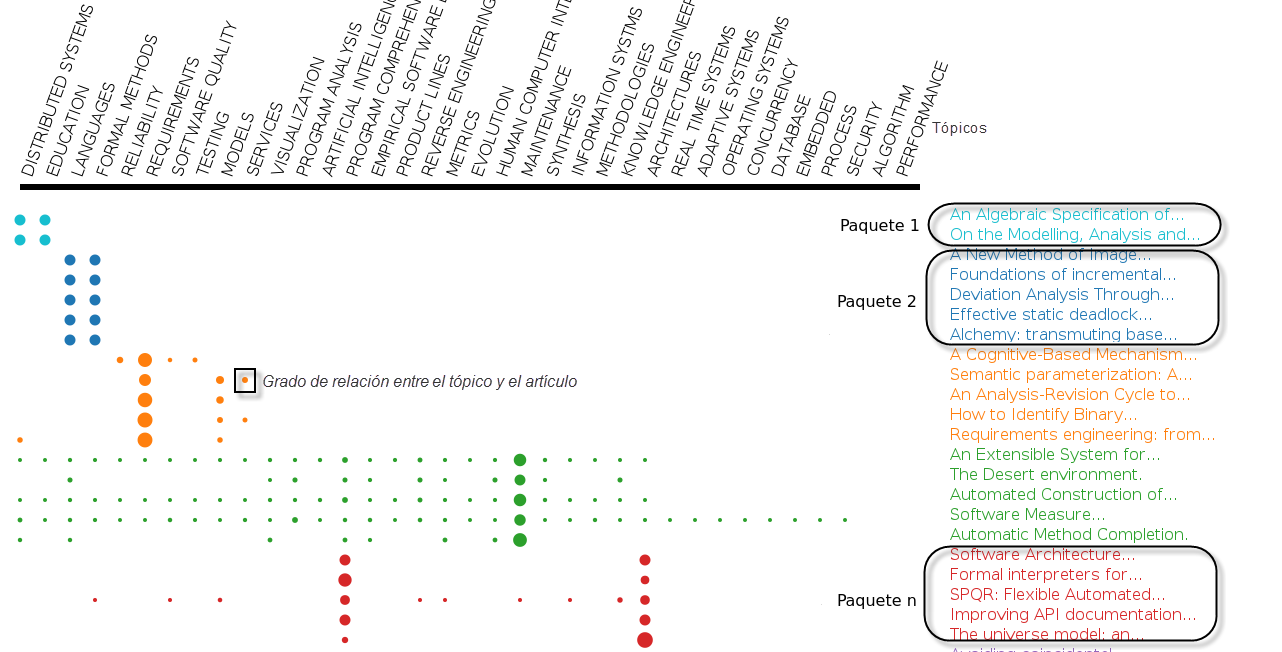
\includegraphics[width=1\textwidth]{img/explain-bars.png}
  \caption{}
  \label{res:img-explain-bars}
\end{figure}

Los gráficos de tipo burbuja de la figura \ref{res:img-explain-bubbles} son útiles para concluir el nivel de acoplamiento entre los paquetes de una solución, observando la relación entre los tópicos y los paquetes. Cada burbuja representa un tópico que contiene círculos; cada circulo es un artículo donde el tamaño es la proporción del articulo con el tópico y el color el paquete al que pertenece. Entonces si las burbujas contienen círculos de más de un color se puede decir que ese resultado no es muy diverso, mientras que el color de los círculos de las burbujas sea más homogéneo el resultado es más diverso. En cuanto a la cohesión de los paquetes, es más cohesivo cuando el tamaño de cada circulo dentro de cada burbuja sea similar (para el mismo color) y la distribución de los círculos entre cada burbuja es equitativa.

\begin{figure}[H]
  \centering
    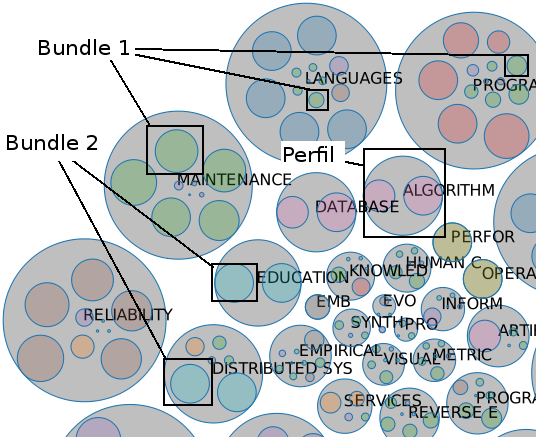
\includegraphics[width=0.5\textwidth]{img/explain-bubbles.png}
  \caption{}
  \label{res:img-explain-bubbles}
\end{figure}

\subsection{Búsqueda de artículos}
Para la búsqueda de artículos con tópicos similares en la tabla \ref{tabla:comp1} se observa los porcentajes de deterioro de cada solución respecto de la mejor solución obtenida por alguno de los ocho algoritmos. Una primera observación es que los algoritmos  Intra-Inter C-HAC reflejan el efecto buscado: a menores valores de $\gamma$ donde el valor inter tiene mayor peso, se obtienen mejores soluciones. Es decir, haber considerado en el proceso de generación de paquetes la funcion Intra-Inter benefició a la calidad de las soluciones obtenidas. Los algoritmos BOBO, no obtienen soluciones de la calidad de los algoritmos C-HAC y el proceso de selección proporcional no logra una mejora consistente para todos los valores de $\gamma$. Las soluciones obtenidas con el algoritmo de construcción golosa, no alcanzaron a mejorar las soluciones de C-HAC pero fueron ampliamente mejores que las de BOBO. En promedio el porcentaje de deterioro de BOBO fue de un $50\%$ mientras que el goloso fue de un $12\%$. 
Cabe resaltar el muy buen rendimiento de la búsqueda tabú, tanto en escenarios donde la solución inicial no es de buena calidad (algoritmo BOBO) así como también considerando soluciones de mejor calidad (algoritmo Intra-Inter C-HAC). En el primer caso, se obtienen porcentajes de mejora por encima del $70\%$. En el segundo caso, para varios valores de $\gamma$ la solución obtenida por la búsqueda tabú resultó ser la mejor opción y en otros con deterioros inferiores al $0.5\%$.
\begin{table}[H]
\begin{center}
\begin{tabular}{|c|c|c|c|c|c|c|c|c|}
\hline
$\gamma$&$alg1$&$alg2$&$alg3$&$alg4$&$alg5$&$alg6$&$alg7$&$alg8$ \\ \hline
0.1 & -2.05 & -32.70 & -36.18 & -7.45 & -0.42 & 0.00 & -4.53 & -3.53 \\
0.2 & -2.11 & -38.06 & -41.19 & -8.23 & 0.00 & 0.00 & -4.92 & -3.85 \\
0.3 & -2.31 & -45.21 & -47.35 & -8.01 & 0.00 & 0.00 & -9.17 & -7.66 \\
0.4 & -0.14 & -49.08 & -51.22 & -15.51 & 0.00 & 0.00 & -10.40 & -9.35 \\
0.5 & 0.00 & -52.35 & -54.23 & -17.87 & -0.31 & -0.31 & -12.97 & -10.38 \\
0.6 & 0.00 & -55.16 & -56.04 & -14.43 & -0.05 & -0.05 & -14.78 & -13.69 \\
0.7 & 0.00 & -56.88 & -56.57 & -17.02 & -0.41 & -0.41 & -16.21 & -15.08 \\
0.8 & 0.00 & -57.86 & -57.86 & -16.11 & -0.56 & -0.30 & -18.10 & -17.60 \\
0.9 & 0.00 & -58.92 & -58.92 & -15.91 & -0.48 & -0.35 & -20.47 & -17.61 \\ \hline 
\end{tabular}
\caption{Comparación de calidad de soluciones entre algoritmos} 
\label{tabla:comp2}
\end{center}
\end{table}

Al comparar las soluciones con mayor y menor función objetivo para los $\gamma = 0,1$ y $\gamma = 0,9$ se observa, en la figura \ref{fig:comp1}, que para $\gamma = 0,1$ los tópicos (representados por burbujas) para la solución de \textit{alg 3} están presentes en varios paquetes (representados por círculos de colores) mientras que para el $alg6$ la mayoría de las burbujas contiene círculos de un solo color. De esta manera se visualiza que la solución de $alg6$ es más diversa. En $\gamma = 0,9$ el resultado obtenido con $alg3$ no se visualiza que cada burbuja contenga cinco circulos del mismo color, en cambio para la solución de $alg1$ si. Eso significa que los paquetes de la solución de $alg1$ son más cohesivos, ya que los cinco elementos de cada paquete tienen los mismos tópicos.

\begin{figure}[H]
	\centering
	\begin{tabular}{cc}
		$alg3$ & $alg6$\\
		\multicolumn{2}{c}{$\gamma=0.1$}\\ 
			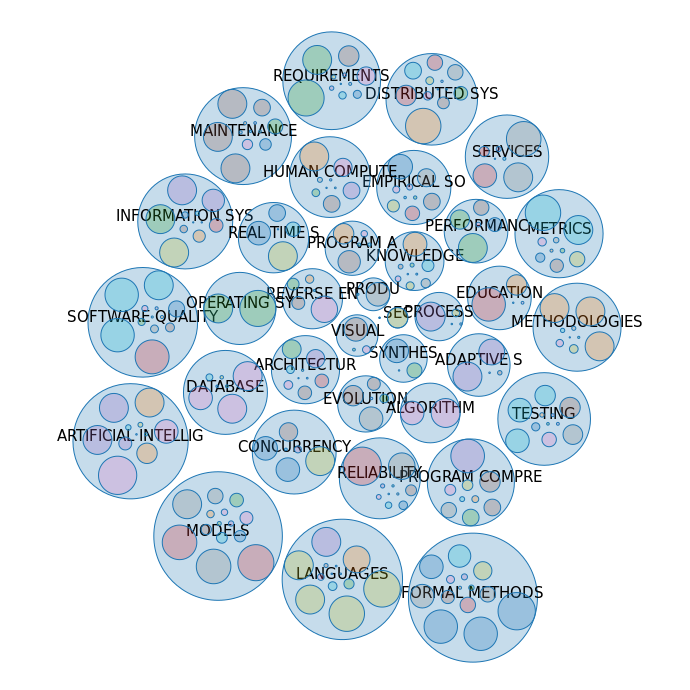
\includegraphics[width=0.5\linewidth]{img/gamma-01-burbujas-alg-3.png}&
			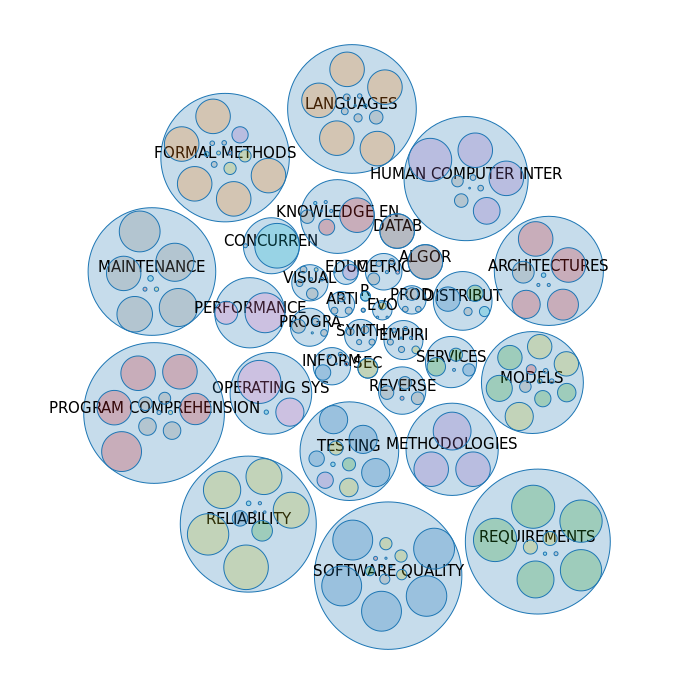
\includegraphics[width=0.5\linewidth]{img/gamma-01-burbujas-alg-6.png} 		\vspace{1cm}\\
			$alg3$ & $alg1$\\
		\multicolumn{2}{c}{$\gamma=0.9$}\\
			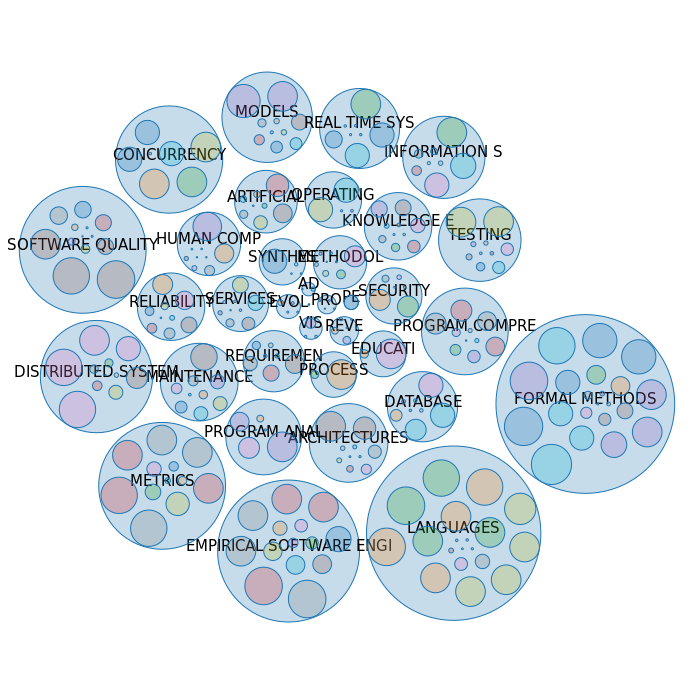
\includegraphics[width=0.5\linewidth]{img/gamma-09-burbujas-alg-3.png}&
			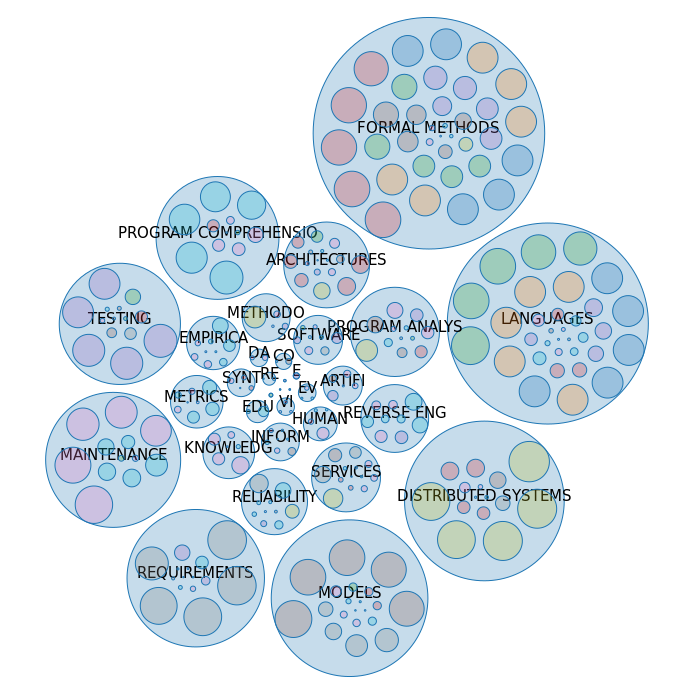
\includegraphics[width=0.5\linewidth]{img/gamma-09-burbujas-alg-1.png}\\
	\end{tabular}
	\caption{Comparación entre las soluciones con menor(izq) y mayor(der) función objetivos  para $\gamma 0,1 y 0,9$}
	\label{res:comp1}
\end{figure}

La búsqueda tabú tiene su mayor impacto cuando es aplicada a la solución brindada por el algoritmo $alg3$ y en este contexto resulta una buena alternativa por su bajo costo computacional.En la Figura~\ref{res:bobo} muestra que para Para $\gamma=0.1$, la solución dada por el $alg3$ tiene artículos de distintos paquetes con patrones muy similares, indicando un bajo valor inter-paquete. Por el contrario, luego de aplicar la búsqueda tabú los patrones de los artículos más similares entre distintos paquetes se volvieron más dispares, demostrando el aumento de la diversidad entre paquetes. Para $\gamma=0.9$, como puede observarse en la misma Figura~\ref{res:bobo}, en la solución brindada por el $alg4$ todos los paquetes tienen al menos un artículo cuyo patrón consiste en muchos pequeños círculos distribuidos en la mayoría de los tópicos en contraposición al resto de los artículos del mismo paquete con pocos círculos de gran tamaño. Esto muestra bajo valor intra-paquete. Mientras que los paquetes obtenidos luego de aplicar la búsqueda tabú son mucho más cohesivos ya que los círculos de los artículos dentro de un mismo paquete siguen patrones mucho más parecidos. Esto demuestra que la búsqueda tabú fue capaz de mejorar las características de la solución en función del parámetro $\gamma$.

Como se mencionó anteriormente, el algoritmo $C-HAC$ de \cite{compositeRetrival} ($alg1$) utiliza la función $Score$ para la decisión del par de {\em clusters} a unir en la etapa de producción de paquetes y la selección simple en la segunda fase. Estos dos criterios omiten la diversidad de los paquetes. De acuerdo a los resultados de la tabla \ref{tabla:comp1}, se pudo concluir que haber considerado la función Intra-Inter y la selección proporcional benefició a la calidad de las soluciones cuando la misma es medida a partir de la función objetivo $w(S)$. Con el fin de evaluar que el $alg5$ es capaz de captar efectivamente la diversidad en la solución, se analiza las soluciones para $\gamma=0.5$. En este caso el $alg1$ obtuvo un valor de $intra=93,82$ y de $inter=35,49$, mientras que el $alg5$ logró valores de $intra=92,94$ y de $inter=35,96$. A pesar de que la solución de $alg1$ es levemente superior, la solución del $alg5$ aumentó el valor $inter$ el $1,32\%$ con un deterioro del valor $intra$ del $0,93\%$. Observando la Figura~\ref{res:chac} se puede ver que la cohesión intra-paquete de ambas soluciones es equivalente. Sin embargo, la diversidad en la segunda solución es mayor, ya que los patrones entre los artículos más similares de distintos paquetes son más heterogéneos. 

\begin{figure}[H]
	\centering
	\begin{tabular}{cc}
		$alg3$ & $alg4$\\
		\multicolumn{2}{c}{$\gamma=0.1$}\\
			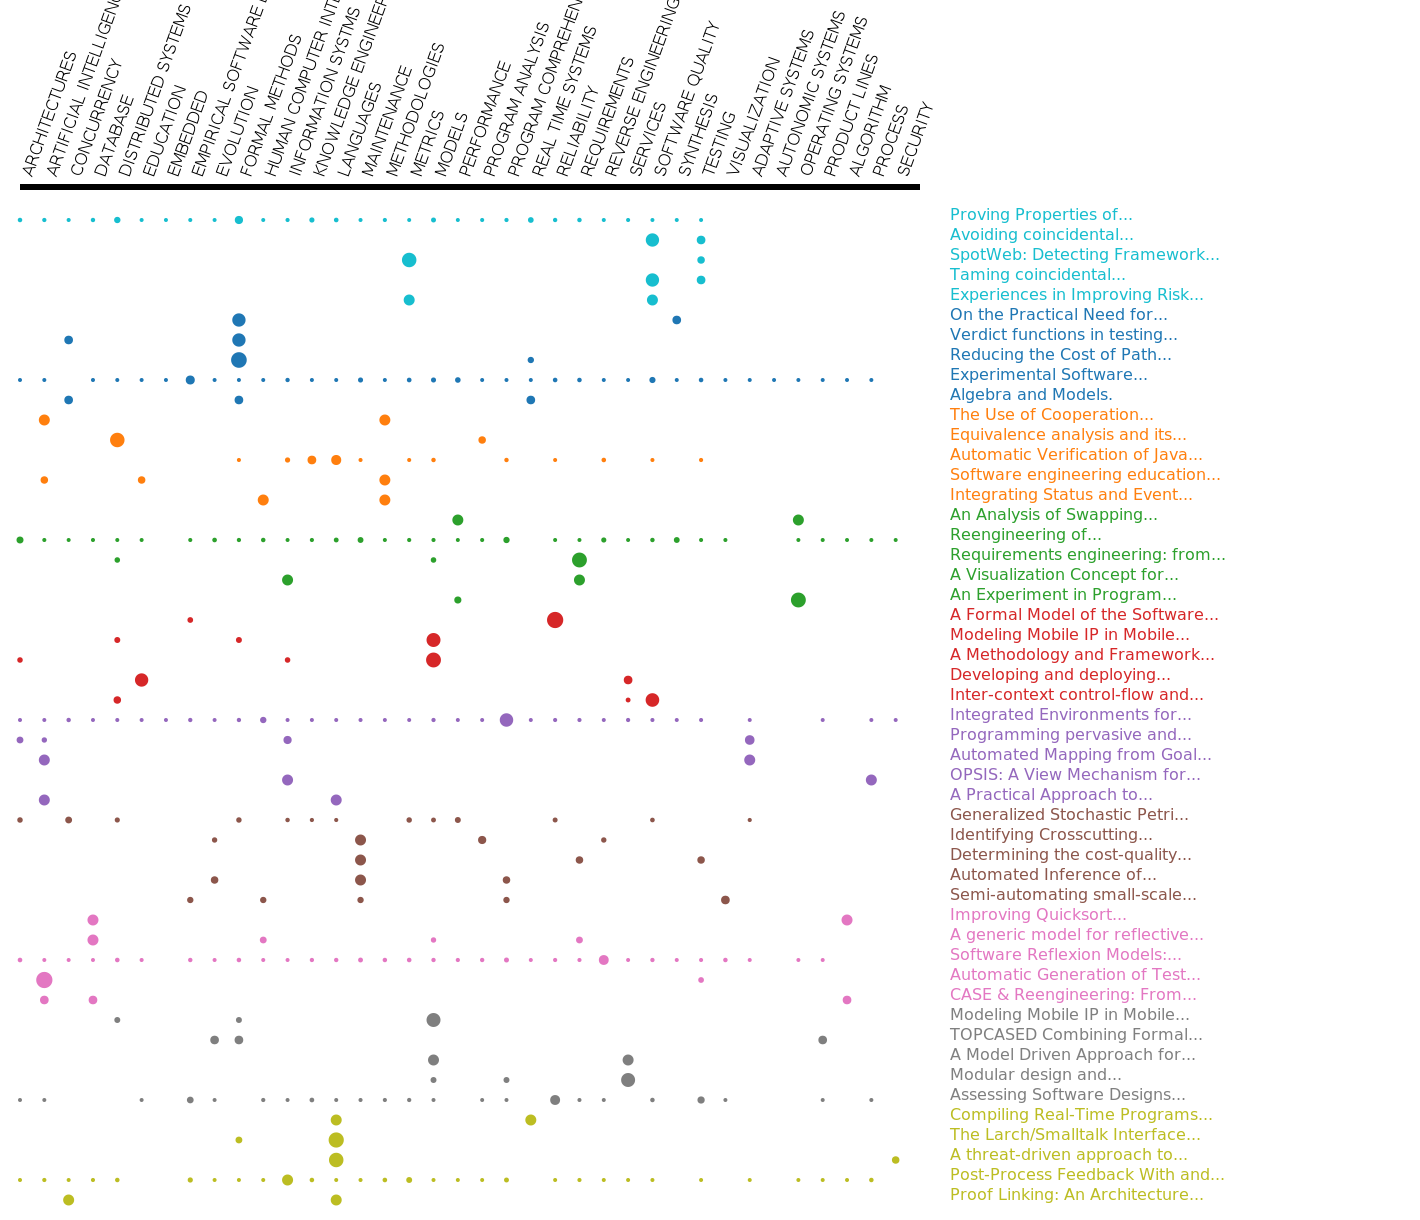
\includegraphics[width=0.5\linewidth]{img/gamma-01-alg-3.png}&
			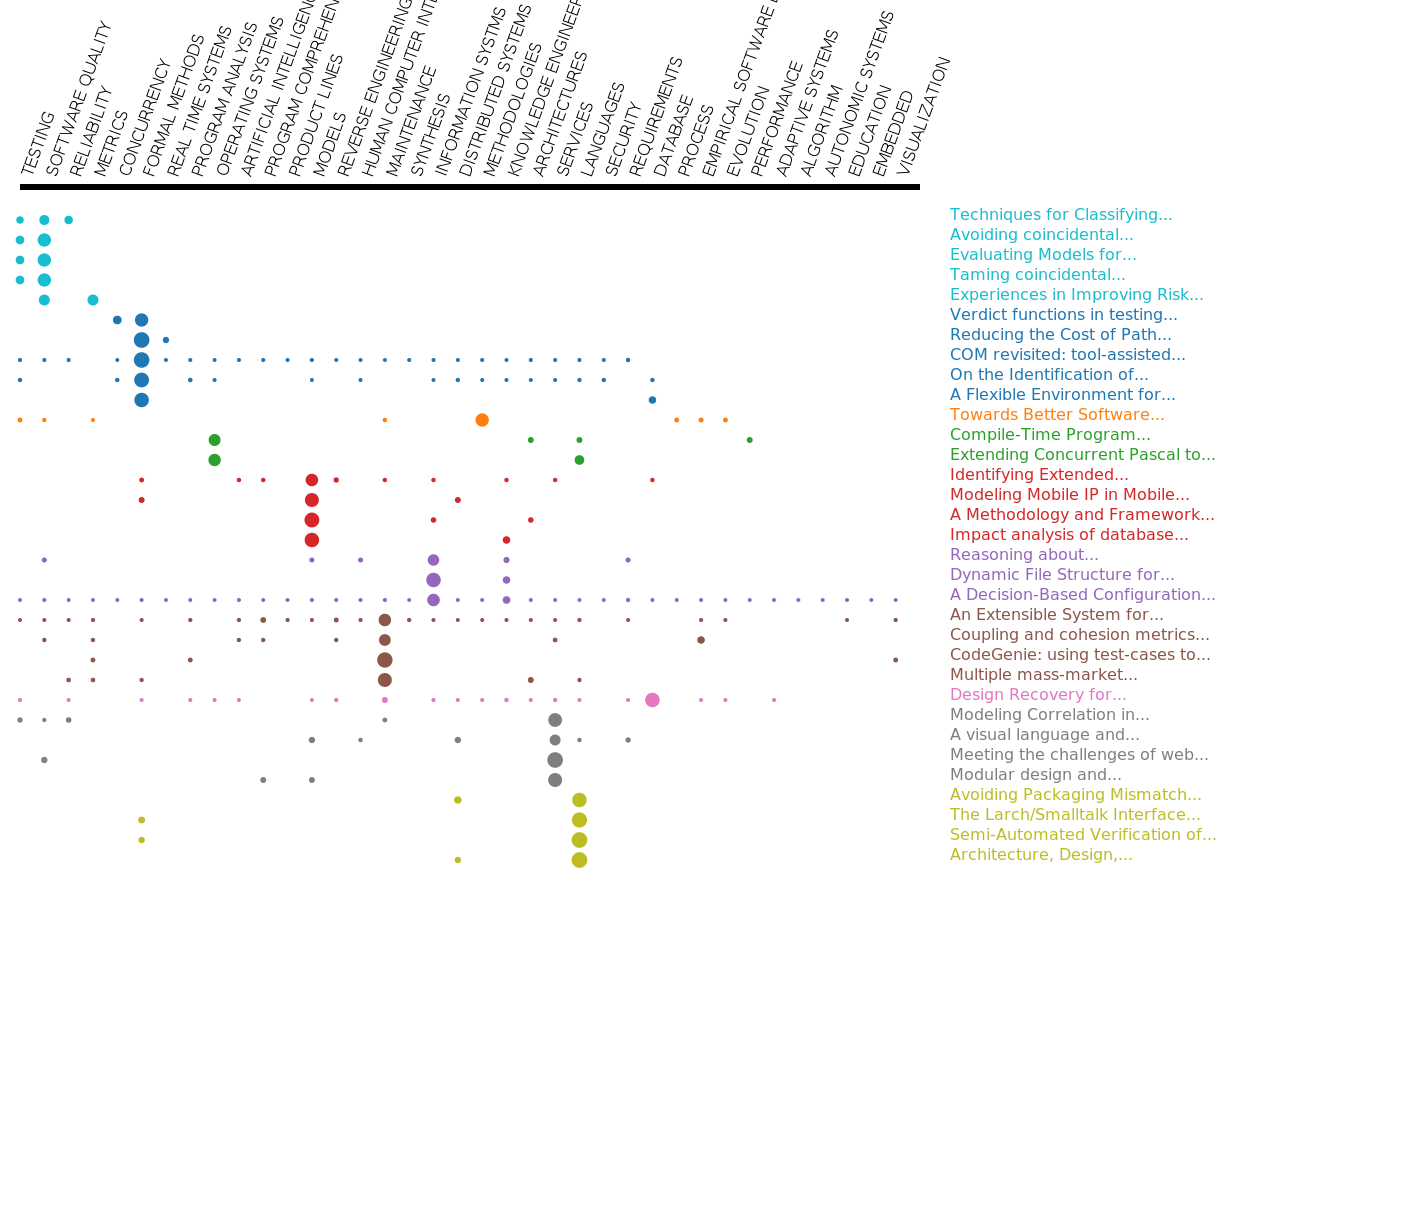
\includegraphics[width=0.5\linewidth]{img/gamma-01-alg-4.png} 		\vspace{1cm}\\
		\multicolumn{2}{c}{$\gamma=0.9$}\\
			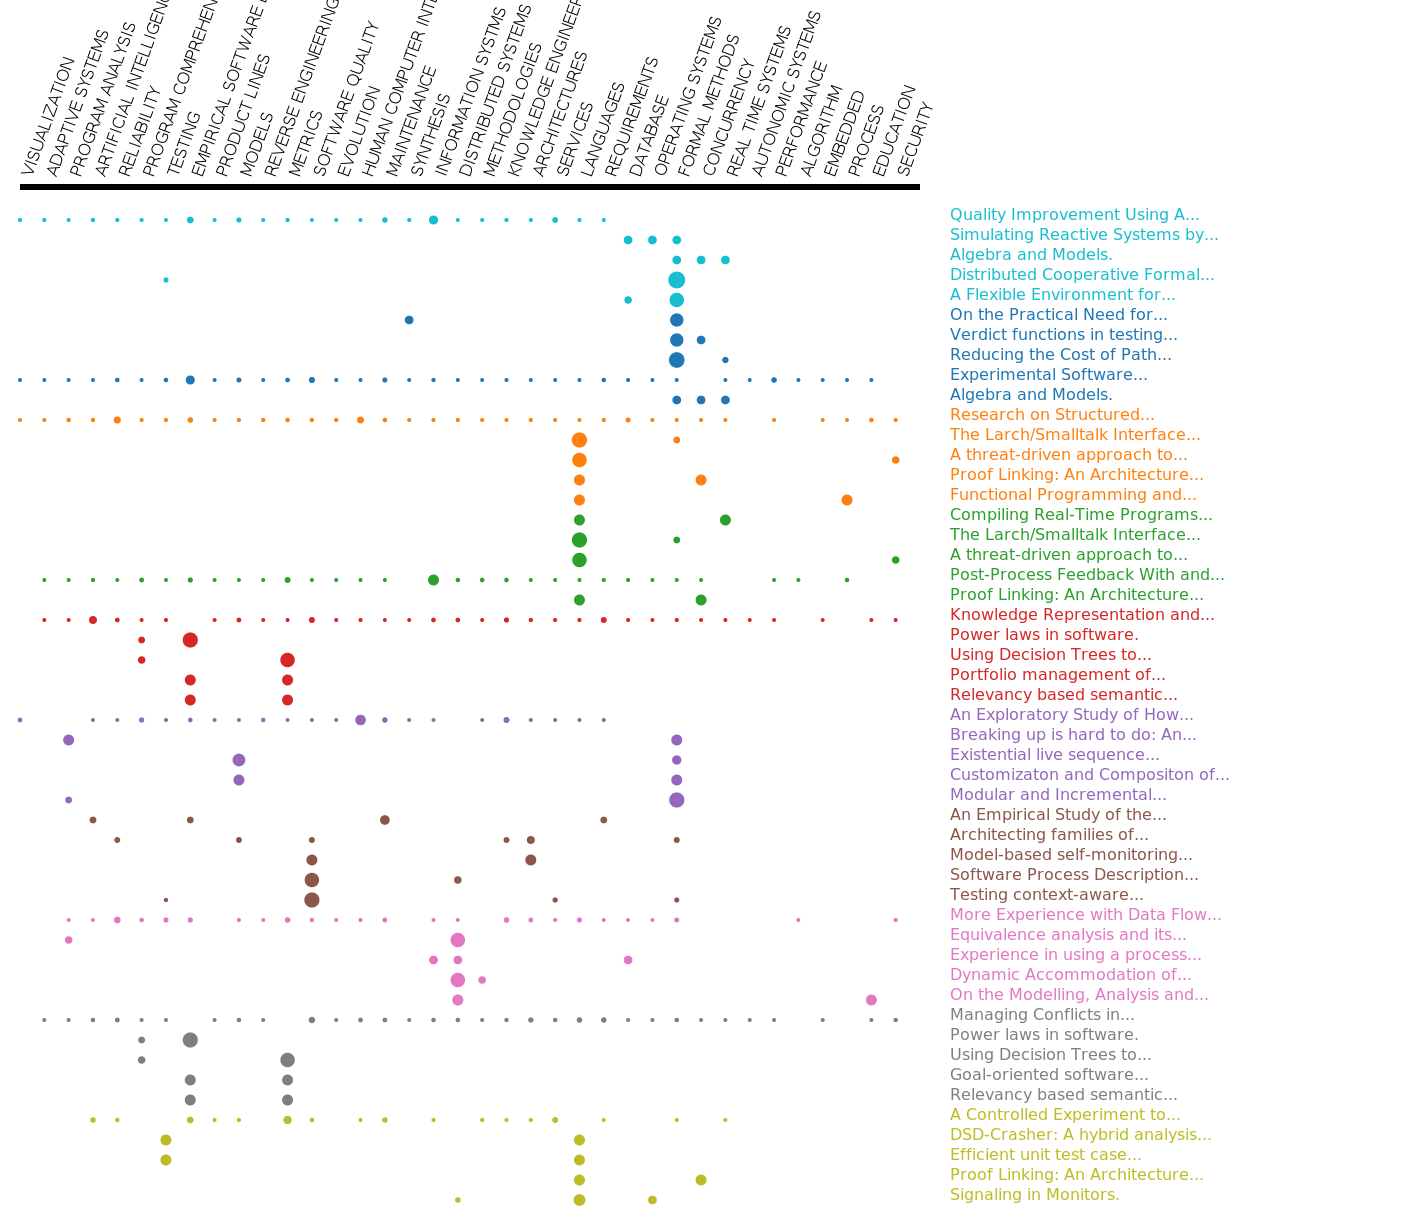
\includegraphics[width=0.5\linewidth]{img/gamma-09-alg-3.png}&
			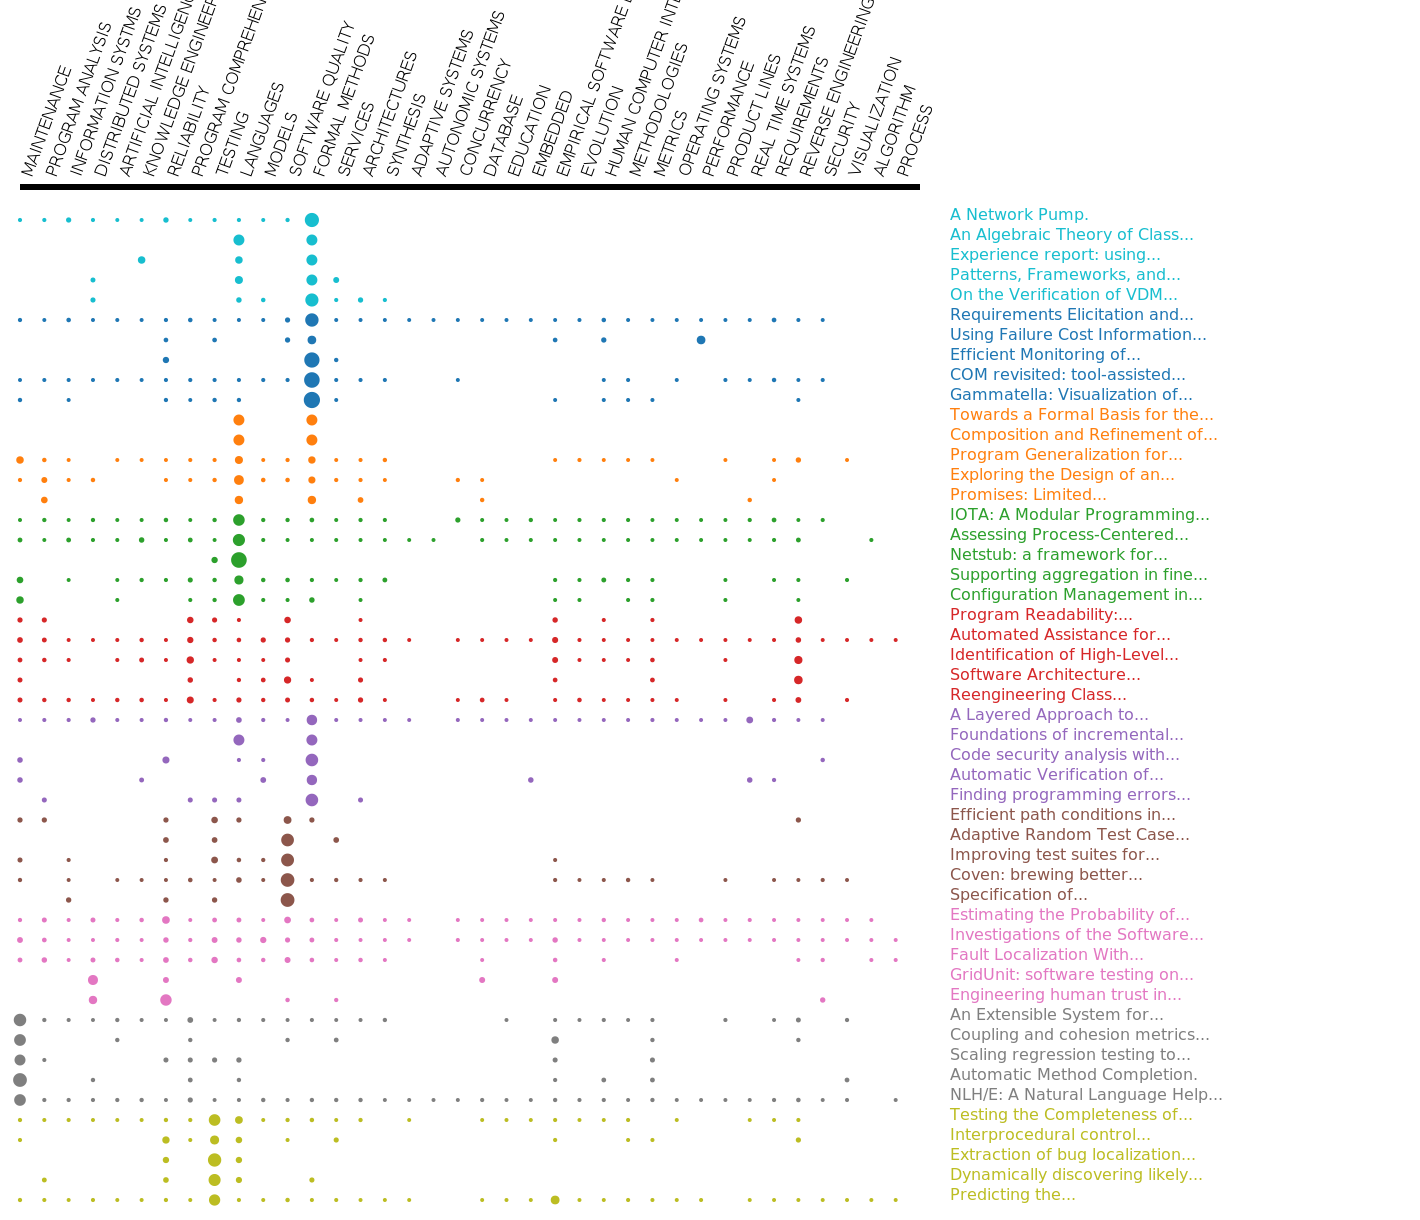
\includegraphics[width=0.5\linewidth]{img/gamma-09-alg-4.png}\\
	\end{tabular}
	\caption{Comparación de soluciones para BOBO-10 con y sin heurística de mejoramiento}
	\label{res:bobo}
\end{figure}

La decisión acerca del valor de $\gamma$ para priorizar un objetivo sobre el otro es realizada por el usuario. Una curva de frontera eficiente podría ayudar para examinar el balance (trade-off) entre los dos objetivos. La intención es que el usuario pueda analizar si una mejora significativa en el valor intra-paquete implica una degradación sustancial en el valor inter-paquetes y viceversa. Para ilustrar este análisis se presenta la Figura \ref{res:inter_intra}  que al comprar las soluciones obtenidas por los algoritmos $alg1$ y $alg5$ variando en pasos de $0,1$. Se observa que las soluciones provistas por $alg5$ no superan en todos los casos el inter en las soluciones obtenidas con $alg1$. En promedio el inter de las soluciones de $alg1$ superan a las de $alg5$ en un $0,65\%$. 

En la misma figura se compara las soluciones obtenidas por el algoritmo goloso $alg7$, que en promedio supera a las soluciones provistas por $alg2$ en $76\%$. De la comparación, se destaca que el valor de $\gamma$ impacta más en las soluciones de $alg2$.  

\begin{figure}[H]
	\centering
	\begin{tabular}{cc}
			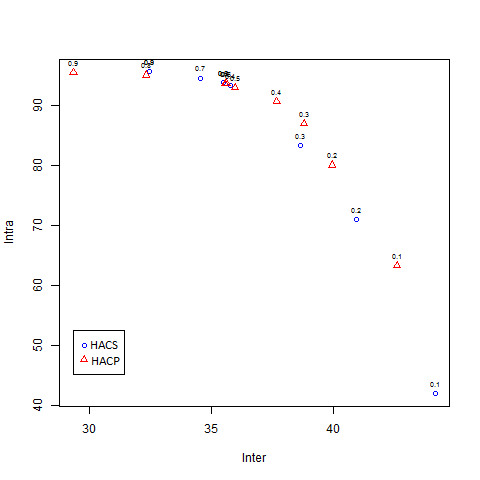
\includegraphics[width=0.5\linewidth]{img/alg1_vs_alg5.png}&
			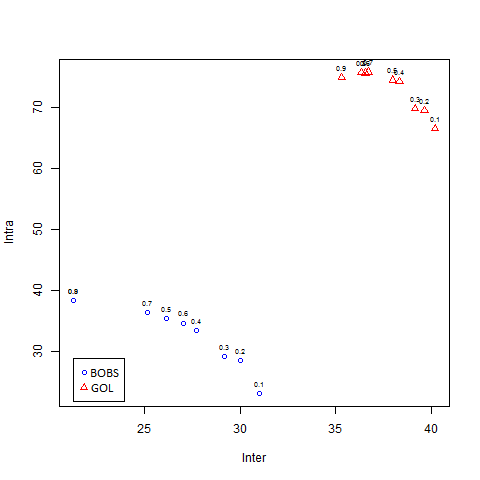
\includegraphics[width=0.5\linewidth]{img/alg2_vs_alg7.png}\\
			$alg1$ vs $alg5$ & $alg2$ vs $alg7$\\
	\end{tabular}
	\caption{}
	\label{res:inter_intra}
\end{figure}

\subsection{Búsqueda de autores}
En la tabla \ref{tabla:comp2} se tiene los porcentajes de deterioro de cada solución para la búsqueda de autores que escribieron artículos de tópicos similares que están afiliados a distintas universidades. Se observa que en este caso, a diferencia de la búsqueda de artículos, el algoritmo tabú no halló una mejor solución.\\
En PAC no hubo una diferencia considerable entre las estrategias de producción $C-HAC$ e $Inter-Intra C-HAC$. Igualmente estos algoritmos jerárquicos siguen demostrando que obtienen una mejor solución que $BOBO$. En cuanto a la etapa de selección, cuando la producción de paquetes se realizó con $BOBO$ no se detecto una mejoría con la estrategia propuesta en este trabajo de la selección proporcional.\\
Al igual que en la búsqueda de artículos, el algoritmo goloso generó para todos los gammas una solución mejor que $BOBO$.\\
En cuanto a la búsqueda tabú, a partir de las soluciones iniciales del algoritmo $alg3$ encontró soluciones en promedio mejor de $30\%$. También encontró mejore soluciones para $alg5$ y $alg7$
\begin{table}[H]
\begin{center}
\begin{tabular}{|c|c|c|c|c|c|c|c|c|}
\hline
$\gamma$&$alg1$&$alg2$&$alg3$&$alg4$&$alg5$&$alg6$&$alg7$&$alg8$ \\ \hline
0.1 & -0.33 & -21.59 & -26.05 & -1.74 & -0.13 & 0.00 & -0.61 & 0.00 \\
0.2 & -0.63 & -27.46 & -29.71 & -0.52 & -0.36 & 0.00 & -1.10 & -0.25 \\
0.3 & -0.44 & -30.57 & -32.47 & -0.20 & -0.53 & 0.00 & -1.50 & -0.34 \\
0.4 & -0.25 & -32.63 & -34.29 & -0.32 & -0.25 & 0.00 & -1.88 & -0.73 \\
0.5 & -0.22 & -34.42 & -35.84 & -0.04 & 0.00 & 0.00 & -2.15 & -0.79 \\
0.6 & -0.18 & -35.86 & -37.05 & -2.01 & 0.00 & 0.00 & -2.45 & -1.39 \\
0.7 & 0.00 & -37.10 & -37.93 & -1.71 & -0.12 & 0.00 & -2.59 & -0.96 \\ 
0.8 & 0.00 & -38.19 & -38.70 & -1.44 & -0.08 & 0.00 & -2.72 & -1.20 \\
0.9 & -0.03 & -39.15 & -39.38 & -1.21 & -0.10 & 0.00 & -3.35 & -1.72 \\ \hline 
\end{tabular}
\caption{Comparación de calidad de soluciones entre algoritmos} 
\label{tabla:comp2}
\end{center}
\end{table}

En la figura \ref{res:aut_alg1_vs_alg5_vs_alg7} de la izquierda se visualiza que los valores inter e intra de las soluciones provistas por el algoritmo $alg2$ para todos los $\gamma$ son significativamente inferiores a las soluciones de los algoritmos $alg1$, $alg5$ y $alg7$. También se observa la pronunciada curva que se genera por el $\gamma$. A la derecha de la misma figura se distingue que las soluciones del algoritmo $alg5$ son más dispersas en la parte inter y están más concentradas en la parte intra que las soluciones del algoritmo $alg1$. En las soluciones del algoritmo $alg5$ la variación entre el mínimo inter y el máximo es $2.12\%$ y para el intra de $0.63\%$ mientras que para $alg1$ la variación es de $0.7\%$ para el inter y de $1.46\%$ para el intra.
\begin{figure}[H]
	\centering
	\begin{tabular}{cc}
			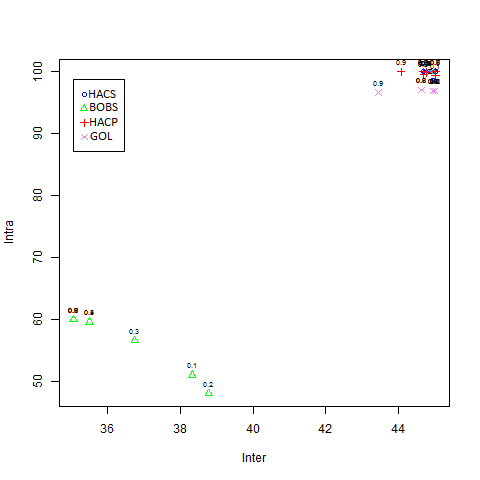
\includegraphics[width=0.5\linewidth]{img/aut-alg1-alg2-alg5-alg7.png}&
			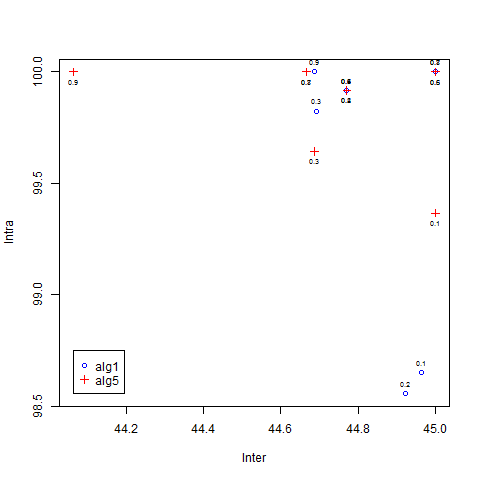
\includegraphics[width=0.5\linewidth]{img/aut-alg1-alg5.png}\\
	\end{tabular}
	\caption{}
	\label{res:aut_alg1_vs_alg5_vs_alg7}
\end{figure}


En esta búsqueda se destaca la búsqueda tabú, principalmente aplicada a la solución obtenida a partir de $alg5$, ya que la solución que se genera para todos los gammas es con el valor máximo posible de la función objetivo con ese presupuesto.

\subsection{Búsqueda de universidades}
En este escenario lo que más se destaca de la tabla \ref{tabla:comp3} es el comportamiento del algoritmo $alg1$ que generó una mejor solución para los valores de $\gamma$ $0.1$ y $0.2$ y para el resto de los valores mayores la solución provista empeora en comparación al algoritmo $alg5$ y la brecha aumenta a medida que aumenta el $\gamma$. 

Por otro lado la función objetivo de las soluciones provista por los algoritmos $alg2$, $alg3$ y $alg7$ se encuentran muy alejadas de las soluciones provistas por los jerárquicos. En el caso del algoritmo goloso $alg7$ las soluciones mejoran con respecto a los algoritmos $alg2$ y $alg3$ cuando el valor de $\gamma$ disminuye.

En este escenario la búsqueda tabú mejoró las soluciones iniciales del BOBO y del algoritmo goloso considerablemente, pero no así con los algoritmos jerárquicos. 
\begin{table}[H]
\begin{center}
\begin{tabular}{|c|c|c|c|c|c|c|c|c|}
\hline
$\gamma$&$alg1$&$alg2$&$alg3$&$alg4$&$alg5$&$alg6$&$alg7$&$alg8$ \\ \hline
0.1 & 0.00 & -30.89 & -31.26 & -15.05 & -1.39 & -1.33 & -10.97 & -9.73 \\
0.2 & 0.00 & -40.35 & -40.16 & -22.09 & -1.72 & -1.07 & -22.83 & -20.42 \\
0.3 & -2.22 & -50.85 & -49.98 & -27.01 & -2.37 & 0.00 & -36.06 & -28.55 \\
0.4 & -5.72 & -60.65 & -58.96 & -33.76 & -1.36 & 0.00 & -48.44 & -30.38 \\
0.5 & -8.59 & -69.76 & -67.66 & -31.46 & -1.92 & 0.00 & -60.18 & -34.32 \\
0.6 & -12.09 & -77.50 & -74.71 & -33.85 & -2.53 & 0.00 & -70.16 & -35.80 \\
0.7 & -12.59 & -82.97 & -80.09 & -31.52 & 0.00 & 0.00 & -78.04 & -29.36 \\
0.8 & -15.52 & -88.12 & -84.93 & -32.90 & 0.00 & 0.00 & -85.63 & -36.34 \\
0.9 & -17.46 & -88.10 & -87.79 & -31.16 & 0.00 & 0.00 & -92.13 & -28.26 \\
 \hline 
\end{tabular}
\caption{Comparación de calidad de soluciones entre algoritmos} 
\label{tabla:comp3}
\end{center}
\end{table}

\section{Búsqueda de atracciones turísticas}\label{res:busAtracciones}
En las búsquedas realizadas sobre la base de datos de atracciones turísticas las soluciones obtenidas a partir de las modificaciones propuestas en este trabajo de los algoritmos PAC mejoran a los originales en todos. Es para destacar que en en este escenario el algoritmo goloso supera a $alg1$. La búsqueda tabú consiguió mejores resultados para los algoritmos PAC, pero no así para el algoritmo goloso.

\begin{table}[H]
\begin{center}
\begin{tabular}{|c|c|c|c|c|c|c|c|c|}
\hline
$\gamma$&$alg1$&$alg2$&$alg3$&$alg4$&$alg5$&$alg6$&$alg7$&$alg8$ \\ \hline
0.1 & -6.49 & -22.89 & -22.30 & -9.99 & -0.05 & 0.00 & -0.52 & -0.52 \\
0.2 & -13.50 & -27.60 & -26.57 & -16.51 & -0.09 & 0.00 & -1.09 & -1.09 \\
0.3 & -21.10 & -32.76 & -29.73 & -20.58 & -0.15 & 0.00 & -1.70 & -1.70 \\
0.4 & -29.38 & -36.68 & -33.51 & -25.10 & -0.20 & 0.00 & -2.37 & -2.37 \\
0.5 & -38.43 & -42.05 & -38.44 & -30.94 & -0.27 & 0.00 & -3.10 & -3.10 \\
0.6 & -48.35 & -47.73 & -43.86 & -34.75 & -0.34 & 0.00 & -3.90 & -3.90 \\
0.7 & -59.29 & -51.47 & -50.54 & -43.46 & -0.41 & 0.00 & -4.78 & -4.78 \\
0.8 & -71.36 & -57.07 & -56.14 & -45.61 & 0.00 & 0.00 & -5.62 & -5.62 \\
0.9 & -84.97 & -60.59 & -59.81 & -44.04 & 0.00 & 0.00 & -7.33 & -7.33 \\
\hline 
\end{tabular}
\caption{Comparación de calidad de soluciones entre algoritmos} 
\label{tabla:comp4}
\end{center}
\end{table}

En la figura \ref{res:cit_bobo_diff} se visualiza el porcentaje de mejora del algoritmo $alg3$ para cada valor de $\gamma$ con respecto a $alg2$. En promedio el porcentaje de mejora es de $3.5\%$ y la mayor diferencia se da para los valores de $\gamma$ $0.3$, $0.4$ y $0.5$
y en los extremos la diferencia disminuye.
\begin{figure}[H]
  \centering
    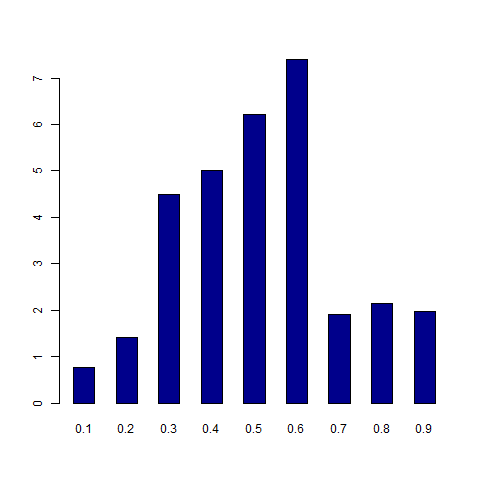
\includegraphics[width=1\textwidth]{img/cit_bobo_diff.png}
  \caption{}
  \label{res:cit_bobo_diff}
\end{figure}
